%
% LaTeX template for prepartion of submissions to PLDI'15
%
% Requires sigplanconf style file provided on PLDI'15 web site
%
\documentclass[pldi]{sigplanconf}

%
% the following standard packages may be helpful, but are not required
%
%\usepackage{SIunits}            % typset units correctly
\usepackage{courier}            % standard fixed width font
\usepackage[scaled]{helvet} % see www.ctan.org/get/macros/latex/required/psnfss/psnfss2e.pdf
\usepackage{url}                  % format URLs
\usepackage{listings}          % format code
\usepackage{enumitem}      % adjust spacing in enums
\usepackage[colorlinks=true,allcolors=blue,breaklinks,draft=false]{hyperref}   % hyperlinks, including DOIs and URLs in bibliography
\usepackage[tight]{subfigure}
\usepackage{xspace}
\usepackage{graphicx}
\usepackage{mathtools}
\usepackage{mathpartir}
\usepackage{amssymb}
\usepackage{amsmath}

\usepackage[usenames,dvipsnames,svgnames,table]{xcolor}
\usepackage{amsthm}
\usepackage[ruled,vlined,linesnumbered]{algorithm2e}
%==============================================================================


\newcommand{\cf}[1]{{\small\tt #1}}
\newcommand{\rcf}[1]{\mathrm{\cf{#1}}}
\newcommand{\conj}{~\wedge~}
\definecolor{darkgreen}{rgb}{0,0.5,0}
\definecolor{darkred}{rgb}{0.5,0,0}
\newcommand{\KC}[1]{{\textcolor{red}{{KC: #1}}}}
\newcommand{\GK}[1]{{\textcolor{red}{{GK: #1}}}}


\lstloadlanguages{sql}
\newcommand{\lstsql}{\lstset{
      language=sql,
      basicstyle=\ttfamily\footnotesize\small,
      flexiblecolumns=false,
      %basewidth={0.5em,0.45em},
      %aboveskip={3pt},
      %belowskip={3pt},
      keywordstyle=\color{blue}\bfseries,
      commentstyle=\color{darkgreen}\itshape,
      % ugh, it keywords map/sort/zipwith.  should do this for
      % consistency or figure out how to disable those other keywords:
      morekeywords={string,REFERENCES}
    }}
\lstnewenvironment{codesql}
    { % \centering
			\lstsql
      \lstset{}%
      \csname lst@setfirstlabel\endcsname}
    { %\centering
      \csname lst@savefirstlabel\endcsname}


\lstloadlanguages{haskell}
\newcommand{\lsthaskell}{\lstset{
      language=haskell,
      basicstyle=\ttfamily\footnotesize\small,
      flexiblecolumns=false,
      %basewidth={0.5em,0.45em},
      %aboveskip={3pt},
      %belowskip={3pt},
      keywordstyle=\color{blue}\bfseries,
      commentstyle=\color{darkgreen}\itshape,
      % ugh, it keywords map/sort/zipwith.  should do this for
      % consistency or figure out how to disable those other keywords:
      morekeywords={foldl,fold,username},
      literate={+}{{$+$}}1 {/}{{$/$}}1 {*}{{$*$}}1 % {=}{{$=$}}1
               {>}{{$>$}}1 {<}{{$<$}}1 {\\}{{$\lambda$}}1
               {\\\\}{{\char`\\\char`\\}}1
               {->}{{$\rightarrow$}}2 {>=}{{$\geq$}}2 {<-}{{$\leftarrow$}}2
               {<=}{{$\leq$}}2 {=>}{{$\rightarrow$}}2
               {\ .}{{$\circ$}}2 {\ .\ }{{$\circ$}}2
               {>>}{{>>}}2 {>>=}{{>>=}}2 {=<<}{{=<<}}2
               {|}{{$\mid$}}1
							 {(-}{{$\in$}}1
               {`member`}{{$\in$}}1
               {s.empty}{{\{\}}}1
               {leftbrace}{\{}1
               {rightbrace}{\}}1
               {profile0sing}{{ \{{\tt profile0}\}}}1
               {\$singleton\$startv}{{ \hspace{2.4em} \{{\tt startv}\}}}1
               {\$singleton\$n}{{  \{{\tt n}\}}}1
               {dotdotdot}{{$\ldots$}}3
    }}
\lstnewenvironment{codehaskell}
    { % \centering
			\lsthaskell
      \lstset{}%
      \csname lst@setfirstlabel\endcsname}
    { %\centering
      \csname lst@savefirstlabel\endcsname}
% known bug: http://tex.stackexchange.com/questions/1522/pdfendlink-ended-up-in-different-nesting-level-than-pdfstartlink
\newcommand{\doi}[1]{doi:~\href{http://dx.doi.org/#1}{\Hurl{#1}}}   % print a hyperlinked DOI

\newcommand{\HA}{{\sf HA}}
\newcommand{\SA}{{\sf SA}}
\newcommand{\UA}{{\sf UA}}
\newcommand{\scc}{\psi_{\sf sc}}
\newcommand{\ccc}{\psi_{\sf cc}}
\newcommand{\ecc}{\psi_{\sf ec}}
\newcommand{\rcc}{\psi_{\sf rc}}
\newcommand{\mavc}{\psi_{\sf mav}}
\newcommand{\rrc}{\psi_{\sf rr}}
\newcommand{\coloneqq}{::=}

\newtheorem{theorem}{Theorem}
\newtheorem{lemma}[theorem]{Lemma}
\newtheorem{proposition}[theorem]{Proposition}
\newtheorem{corollary}[theorem]{Corollary}
\newtheorem{definition}[theorem]{Definition}
\newcounter{hno}
\newcounter{gno}
\renewenvironment{proof}{\setcounter{hno}{0}\setcounter{gno}{0}
  \emph{Proof.}}{}
\newcommand{\npp}{\thehno \stepcounter{hno}}
\newcommand{\mpp}{\thegno \stepcounter{gno}}

\newcommand{\stretcharraybig}{\renewcommand*{\arraystretch}{1.25}}
\newcommand{\cureff}{\hat{\eta}}
\newcommand{\eff}{\eta}
\newcommand{\fresh}{\N{\sf fresh}}
\newcommand{\cv}{\psi}
\newcommand{\ALT}{~\mid~}
\newcommand{\eid}{{\iota}}
\newcommand{\ObjType}{{\sf ObjType}}
\newcommand{\AbsType}{{\sf AbsType}}
\newcommand{\dom}{{\sf dom}}
\newcommand{\DtLib}[1]{\mathbb{D}(#1)}
\newcommand{\DtLibZ}{\mathbb{D}}
\newcommand{\Ops}{\Lambda}
\newcommand{\Ctrts}{\Psi}
\newcommand{\true}{\N{\textsf{true}}}

\newcommand{\R}[1]{\textrm{#1}}
\newcommand{\N}[1]{{\normalfont #1}}
\newcommand{\ObjZ}{\N{\textsf{Obj}}}
\newcommand{\Obj}[1]{\N{\textsf{Obj}_{#1}}}
\newcommand{\ReplID}{\mathtt{ReplID}}
\newcommand{\SessID}{\mathtt{SessID}}
\newcommand{\typeFun}[1]{\N{\textsf{type}}(#1)}
\newcommand{\Op}[1]{\N{\textsf{Op}_{#1}}}
\newcommand{\set}[1]{\overline{#1}}
\newcommand{\unitVal}{\N{\textsf{unit}}}
\newcommand{\EffUniv}{\N{\sf Effect}}
\newcommand{\EffID}{\mathtt{SeqNo}}
\newcommand{\TransID}{\N{\sf TransID}}
\newcommand{\AVal}[1]{\N{\textsf{AVal}_{#1}}}
\newcommand{\RVal}[1]{\N{\textsf{RVal}_{#1}}}
\newcommand{\Eff}[1]{\N{\textsf{Eff}_{#1}}}
\newcommand{\loud}[1]{\textbf{\textit{#1}}}
\newcommand{\dt}[1]{\mathcal{D}_{#1}}
\newcommand{\vis}[2]{\N{\textsf{vis}(#1,#2)}}
\newcommand{\visZ}{\N{\textsf{vis}}}
\newcommand{\Rvis}{\N{\textsf{vis}}}
\newcommand{\arZ}{\N{\textsf{ar}}}
\newcommand{\ar}[2]{\N{\textsf{ar}(#1,#2)}}
\newcommand{\stxZ}{\sim}
\newcommand{\stx}[2]{#1\sim#2}
\newcommand{\nstx}[2]{#1\not\sim#2}
\newcommand{\comZ}{\N{\textsf{com}}}
\newcommand{\com}[1]{\comZ(#1)}
\newcommand{\so}[2]{\N{\textsf{so}(#1,#2)}}
\newcommand{\soZ}{\N{\textsf{so}}}
\newcommand{\stZ}{\N{\textsf{st}}}
\newcommand{\Rso}{\N{\textsf{so}}}
\newcommand{\Rst}{\N{\textsf{st}}}
\newcommand{\COM}{\textrm{\sc {\small Commit}}}
\newcommand{\soo}[2]{\N{\textsf{soo}(#1,#2)}}
\newcommand{\sooZ}{\N{\textsf{soo}}}
\newcommand{\hb}[2]{\N{\textsf{hb}(#1,#2)}}
\newcommand{\hbo}[2]{\N{\textsf{hbo}(#1,#2)}}
\newcommand{\hbZ}{\N{\textsf{hb}}}
\newcommand{\hboZ}{\N{\textsf{hbo}}}
\newcommand{\oper}[2]{\N{\textsf{oper}(#1,#2)}}
\newcommand{\operZ}{\N{\textsf{oper}}}
\newcommand{\txnZ}{\N{\textsf{txn}}}
\newcommand{\txn}[2]{\txnZ\{#1\}\{#2\}}
\newcommand{\sameobj}[2]{\N{\textsf{sameobj}(#1,#2)}}
\newcommand{\sameobjZ}{\N{\textsf{sameobj}}}
\newcommand{\sametxn}[2]{\N{\textsf{sametxn}(#1,#2)}}
\newcommand{\sametxnZ}{\N{\textsf{sametxn}}}
\newcommand{\E}{\N{\textsf{E}}}
\newcommand{\EffSoup}{\N{\textsf{A}}}
\newcommand{\obj}{\N{\textsf{obj}}}
\newcommand{\dep}{\N{\textsf{dep}}}
\newcommand{\rval}{\N{\textsf{rval}}}
\newcommand{\repl}{\N{\textsf{repl}}}
\newcommand{\sess}{\N{\textsf{sess}}}
\newcommand{\rdtspec}{\Delta}
\newcommand{\goesto}{\longrightarrow}
\newcommand{\tuplee}[1]{\langle #1 \rangle}
\newcommand{\ctxtFn}{\N{\textsf{ctxt}}}
\newcommand{\rdtredsto}{\N{\leadsto}}
\newcommand{\Exec}{\N{\textsf{(\EffSoup,\allowbreak \visZ,\allowbreak \soZ,\allowbreak \sameobjZ)}}}
\newcommand{\pll}{~\|~}
\newcommand{\Mod}[1]{\N{\textsf{Mod}}(#1)}
\newcommand{\De}[1]{[\![#1]\!]}
\newcommand{\Der}[2]{[\![#1,#2]\!]_{r}}
\newcommand{\msentails}[2]{#1 \models #2}
\newcommand{\hasTyp}[2]{#1 \vdash #2}
\newcommand{\auxred}[4]{#1 #2 \;\xrightarrow{#3}\; #4 }


% Operational semantics rules
\newcommand{\rulelabel}[1]{\textrm{\sc {\small [#1]}}}
\newcommand{\RULE}[3]
{\frac{\begin{array}{c}#1\end{array}}
		 {\begin{array}{c}#2\end{array}}
~ \rulelabel{#3}
}

\newcommand{\RuleTwo}[2]
{\frac{\begin{array}{c}#1\end{array}}
		 {\begin{array}{c}#2\end{array}}
}

\newenvironment{nop}{}{}
\newenvironment{smathpar}{
\begin{nop}\small\begin{mathpar}}{
\end{mathpar}\end{nop}\ignorespacesafterend}

\newcommand{\rsf}[1]{\R{\sf #1}}
\newcommand{\trans}[4]{\N{\textsf{trans}}\{#1,#2\}\{#3,#4\}}

\newcommand{\name}{{\sc Quelea}\xspace}


%% KC spacing edits -- should be removed eventually -- Fix the text!
\setlength{\floatsep}{5pt}
\setlength{\textfloatsep}{10pt}
\setlength{\dblfloatsep}{5pt}
\setlength{\dbltextfloatsep}{10pt}



\begin{document}

%
% any author declaration will be ignored  when using 'plid' option (for double blind review)
%

\title{Declarative Programming over Eventually Consistent Data Stores }

\maketitle
\begin{abstract}
User-facing online services utilize geo-distributed data stores to minimize
latency and tolerate partial failures, with the intention to provide a fast,
always-on experience. However, geo-distribution does not come for free;
application developers have to contend with weak consistency behaviors, and
the lack of abstractions to composably construct high-level replicated data
types, necessitating the need for complex application logic and invariably
exposing inconsistencies to the user. Some commercial distributed data
stores and several academic proposals do propose to provide a lattice of
consistency levels, with stronger consistency at the cost of latency and
throughput. However, correctly assigning the consistency level for an
operation is a error-prone task.

In this paper, we present \name, a declarative programming model for
eventually consistent data stores, equipped with a \emph{contract} language,
capable of specifying fine-grained application-level consistency
properties. A \emph{contract enforcement system} analyses contracts, and
automatically generates the appropriate consistency protocol for the method
protected by the contract. We describe an implementation of \name\ on top of
an off-the-shelf eventually consistent data store, and provide support for
\emph{coordination-free} transactions. Several benchmarks including two
large web applications, illustrate the effectiveness of our approach.
\end{abstract}

\section{Introduction}

Many real-world web services --- such as those built and maintained by Amazon,
Facebook, Google, Twitter, etc. --- replicate application state and logic
across multiple \emph{replicas} within and across data centers. Replication is
intended not only to improve application throughput and reduce user-perceived
latency, but also to tolerate partial failures without compromising overall
service availability. Traditionally programmers have relied on \emph{strong
consistency} guarantees such as linearizability~\cite{Herlihy1990} or
serializability~\cite{Serializability} in order to build correct applications.
While strong consistency is an easily stated property, it masks the reality
underlying large-scale distributed systems with respect to non-uniform latency,
availability and network partitions~\cite{Brewer2000,Gilbert2002}. Indeed,
modern web services, which aim to provide an "always-on" experience,
overwhelmingly favor availability and partition tolerance over strong
consistency. To this end, several \emph{weak consistency} models such as
eventual consistency, causal consistency, session guarantees, and timeline
consistency have been proposed.

Under weak consistency, the developer needs to be aware of concurrent
conflicting updates, and has to pay careful attention to avoid unwanted
inconsistencies (e.g., negative balances in a bank account, or having an item
appear in a shopping cart after it has been removed~\cite{Dynamo}). Oftentimes,
these inconsistencies leak from the application and is witnessed by the user.
Ultimately, the developer must decide the consistency level appropriate for a
particular operation; this is understandably an error-prone process requiring
intricate knowledge of both the application as well as the semantics and
implementation of the underlying data store, which typically have only informal
descriptions. Nonetheless, picking the correct consistency level is critical
not only for correctness but also for scalability of the application. While
choosing a weaker consistency level than required may introduce program errors
and anomalies, choosing a stronger one than necessary can negatively impact
program scalability and performance.

Weak consistency also hinders compositional reasoning about programs.  Although an
application might be naturally expressed in terms of well-understood and
expressive data types such as maps, trees, queues, or graphs, geo-distributed
stores typically only provide a minimal set of data types with in-built
conflict resolution strategies such as last-writer-wins (LWW) registers,
counters, and sets~\cite{Cassandra,DynamoDB}.  Furthermore, while traditional
database systems enable composability through transactions, geo-distributed
stores typically lack unrestricted serializable transactional access to the
data. Working in this environment thus requires application state to be
suitably coerced to function using only the capabilities of the store.

To address these issues, we describe \name, a declarative programming model and
implementation for eventually consistent geo-distributed data stores. The key
novelty of \name is an expressive \emph{contract language} to declare and
verify fine-grained application-level consistency properties. The programmer
uses the contract language to axiomatically specify the set of legal executions
allowed over the replicated data type. Contracts are constructed using
primitive consistency relations such as \emph{visibility} and \emph{session
order} along with standard logical and relational operators. A \emph{contract
enforcement system} statically maps operations over the datatype to a
particular consistency level available on the store, and provably validates the
correctness of the mapping. The paper makes the following contributions:
\vspace*{-.4em}
\begin{itemize}
\setlength{\itemsep}{2pt}
\item We introduce \name, a shallow extension of Haskell that supports the
	description and validation of replicated data types found on eventually
	consistent stores. Contracts are used to specify fine-grained
	application-level consistency properties, and are statically analyzed to
	assign the most efficient and sound store consistency level to the
	corresponding operation.
\item \name supports coordination-free transactions over arbitrary datatypes.
	We extend our contract language to express fine-grained transaction isolation
	guarantees, and utilize the contract enforcement system to automatically
	assign the correct isolation level for a transaction.
\item We provide meta-theory that certifies the soundness of our contract
	enforcement system, and ensures that an operation is only executed if the
	required conditions on consistency are met.
\item An implementation of \name as a transparent shim layer over
	Cassandra~\cite{Cassandra}, a well-known general-purpose data store.
	Experimental evaluation over a set of real-world applications, including a
	Twitter-like micro-blogging site and an eBay-like auction site illustrates
	the practicality of our approach.
\end{itemize}

\noindent The rest of the paper is organized as follows. The next section
describes the system model.  We describe the challenges in programming with
eventually consistent data stores, and introduce \name\ contracts as a proposed
solution to overcome these issues in \S~\ref{sec:motivation}. \S~\ref{sec:lang}
provides more details on the contract language, and its mapping to the store
consistency levels, along with meta-theory for certifying the correctness of
the mapping. \S~\ref{sec:txns} introduces transaction contracts and their
classification. \S~\ref{sec:impl} describes the implementation of \name on top
of Cassandra. \S~\ref{sec:results} discusses experimental evaluation.
\S~\ref{sec:related} and~\ref{sec:concl} present related work and conclusions.


\section{Motivation}
\label{sec:motivation}

Consider how we might implement a highly available bank account on top of an
\ecds, with the \emph{integrity} constraint that the balance must be
non-negative. We begin by implementing a bank account replicated data type
(RDT) in \name, and then describe the mechanisms to obtain the desired
correctness guarantees.

\subsection{RDT specification}

A key novelty in \name is that it allows the addition of new RDTs to the store,
which obviates the need for coercing the application logic to utilize the store
provided data types. In addition, \name treats the convergence semantics (i.e.,
\emph{how} conflicting updates are resolved) of the data type separately from
its consistency properties (i.e., \emph{when} updates become visible). This
separation of concerns permits \emph{operational} reasoning for conflict
resolution, and \emph{declarative} reasoning for consistency. The combination
of these techniques enhances the programmability of the store.

Let us assume that the bank account object provides three operations:
\cf{deposit}, \cf{withdraw} and \cf{getBalance}, with the assumption that the
withdraw fails if the account has insufficient balance. Every operation in
\name is of the following type, written in Haskell syntax:

\begin{codehaskell}
type Operation e a r = [e] -> a -> (r, Maybe e)
\end{codehaskell}

\noindent It takes a list of effects (the \emph{history} of updates to that
object), and an input argument, and returns a result along with an optional
effect (read-only operations return \cf{Nothing}). The new effect (if emitted)
is added to the state of the object at the current replica, and asynchronously
sent to other replicas. The implementation of the bank account operations in
\name is given in Figure~\ref{fig:ex}.

\begin{figure}
\vspace{-2.3mm}
\begin{codehaskell}
data Acc = Deposit Int | Withdraw Int | GetBal

getBalance :: [Acc] -> () -> (Int, Maybe Acc)
getBalance hist _ =
  let res = sum [x | Deposit x <- hist]
						- sum [x | Withdraw x <- hist]
	in (res, Nothing)

deposit :: [Acc] -> Int -> ((), Maybe Acc)
deposit hist amt = ((), Just dollar Deposit amt)

withdraw :: [Acc] -> Int -> (Bool, Maybe Acc)
withdraw hist v =
	if sel1 dollar getBalance hist () >= v
  then (True, Just dollar Withdraw v)
	else (False, Nothing)
\end{codehaskell}
\caption{Definition of a bank account expressed in Quelea.}
\label{fig:ex}
\end{figure}

The datatype \cf{Acc} represents the effect type for the bank account. The
function \cf{sum} returns the sum of elements in the list, and \cf{sel1}
returns the first element of a tuple. For each operation, \cf{hist} is a
\emph{snapshot} of the state of the object at some replica. In this sense,
every operation on the RDT is atomic, and thus permitting sequential reasoning
for implementing the RDTs. Here, \cf{getBalance} is a read-only operation,
\cf{deposit} always emits an effect, and \cf{withdraw} only emits an effect if
there is sufficient balance in the account. We have implemented a large corpus
of RDTs for realistic benchmarks including shopping carts, auction and
micro-blogging sites in few tens of lines of code.

\subsubsection{Summarization}
\label{sec:summarize}

Observe that the definition of \cf{getBalance} reduces over the \emph{entire
history} of updates to an account. If we are to realize an efficient
implementation of this bank account RDT, we need a \emph{summary} of the
account history. Intuitively, the current account balance summarizes the state
of an account. A bank account with the history \cf{[Deposit 10, Withdraw 5]} is
\emph{observably equivalent} to a bank account with a single deposit operation
\cf{[Deposit 5]}; we can replace the earlier history with the latter and a
client of the store would not able to tell the difference between the two.

This notion of observable equivalence can be generalized to other RDTs as well.
For example, a last-writer-wins register with multiple updates is equivalent to
a register with only the last write. Similarly, a set with a collection of add
and remove operations is equivalent to a set with a series of additions of live
elements from the original set. Since the notion of observable equivalence is
specific to each RDT, we expect the programmer to provide a summarization
function (\cf{summarize}) of type \cf{[e] -> [e]} for each RDT, as a part of
the RDT specification.

The summarization function for the bank account is \cf{summarize hist =
[Deposit \$ sel1 \$ getBalance hist ()]}. Given a bank account history
\cf{hist}, the \cf{summarize} function returns a new history with a single
deposit of the current account balance. We utilize the summarization function
to ensure that the state of an object remains summarized in each replica.

\subsection{Anomalies under Eventual Consistency}

Our goal is to choose the correct consistency level for each of the bank
account operations such that (1) the balance remains non-negative and (2) the
\cf{getBalance} operation never incorrectly returns a negative balance.

\begin{figure}[ht]
\vspace{-2mm}
\centering
\subfigure[Unsafe withdraw]{\label{fig:unsafeWithdrawAnomaly}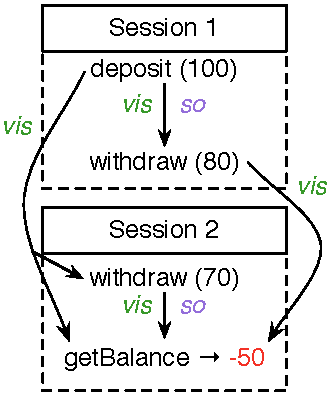
\includegraphics[width=0.34\columnwidth]{Figures/Motivation4}}
\hfill
\subfigure[Negative balance]{\label{fig:negativeBalanceAnomaly}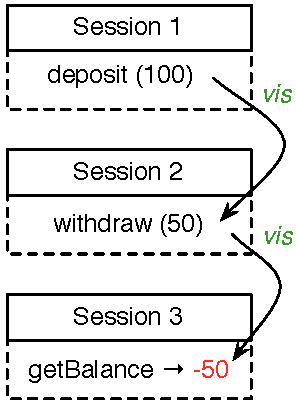
\includegraphics[width=0.31\columnwidth]{Figures/Motivation2}}
\hfill
\subfigure[Missing update]{\label{fig:missingUpdateAnomaly}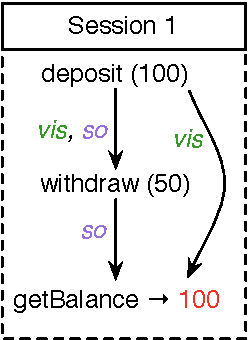
\includegraphics[width=0.26\columnwidth]{Figures/Motivation1}}
\caption{Anomalies possible under eventual consistency for the get balance operation.}
\label{fig:ba_anomalies}
\end{figure}

Consider the execution shown in Figure~\ref{fig:unsafeWithdrawAnomaly}. Assume
that all operations in the figure are on the same bank account object with the
initial balance being zero. Session 1 performs a \cf{deposit} of 100, followed
by a \cf{withdraw} of 80 in the same session. The \cf{withdraw} operation
witnesses\footnote{Although visibility and session
order relations relate effects, we have abused the notation in these examples
to relate operations, with the idea that the relations relate the effect
emitted by those operations} the deposit and succeeds. Subsequently, session 2 perform a \cf{withdraw}
operation, but importantly, due to eventual consistency, only witnesses the
\cf{deposit} from session 1, but not the subsequent withdraw. Hence, this
\cf{withdraw} also \emph{incorrectly} succeeds, violating the integrity
constraint. A subsequent \cf{getBalance} operation, that happens to witness all
the previous operations, would report a negative balance.

It is easy to see that preventing concurrent \cf{withdraw} operations
eliminates this anomaly. This can be done by insisting that \cf{withdraw} be
executed as a strongly consistent operation. Despite this strengthening,
the \cf{getBalance} operation may still incorrectly report a negative balance to
the user. Consider the execution shown in
fig.~\ref{fig:negativeBalanceAnomaly}, which consists of three concurrent
sessions performing a \cf{deposit}, a \cf{withdraw}, and a \cf{getBalance}
operation, respectively, on the same bank account object. As the {\sf vis} edge
indicates, operation \cf{withdraw(50)} in session 2 witnesses the effects of
\cf{deposit(100)} from session 1, concludes that there is sufficient balance,
and completes successfully. However, the \cf{getBalance} operation may only
witness this successful withdraw, but not the causally preceding \cf{deposit},
and reports the balance of negative 50 to the user.

Under eventual consistency, the users may also be exposed to other forms of
inconsistencies. Figure~\ref{fig:missingUpdateAnomaly} shows an execution where
the \cf{getBalance} operation in a session does not witness the effects of an
earlier \cf{withdraw} operation performed in the same session, possibly because
it was served by a replica that has not yet merged the \cf{withdraw} effect.
This anomaly leads the user to incorrectly conclude that the \cf{withdraw}
operation failed to go through.

Although it is easy to understand the reasons behind the occurrence of the
aforementioned anomalies, finding the appropriate fixes is not readily
apparent. Making \cf{getBalance} a strongly consistent operation is definitely
sufficient to avert anomalies, but is it really necessary? Given the cost of
enforcing strong consistency~\cite{DynamoDB, Pileus}, it is preferable to avoid
it unless there are no viable alternatives. Exploring the space of these
alternatives requires understanding the subtle differences in semantics of
various kinds of weak consistency alternatives.

\subsection{Contracts}

\name helps facilitate the mapping of operations to appropriate consistency
levels by letting the programmer declare application-level consistency
constraints as \emph{contracts}\footnote{\name exposes the contract
construction language as a Haskell library} (Figure~\ref{fig:contract-lang})
that axiomatically specify the set of allowed executions involving this
operation. In the case of the bank account, any execution that does not exhibit
the anomalies described in the previous section is a \emph{well-formed}
execution on the bank account object. By specifying the set of legal executions
for each data type in terms of a trace of operation invocations on that type,
\name\ ensures that all executions over that type are well-formed.

In our running example, it is clear that in order to preserve the integrity
constraint, the \cf{withdraw} operation must be strongly consistent.  That is,
given two \cf{withdraw} operations $a$ and $b$, either $a$ is visible to $b$ or
vice-versa. We express this application-level consistency requirement as a
contract ($\cv_w$) over \cf{withdraw}:

\vspace{-1em}
\begin{smathpar}
\begin{array}{l}
\forall (a : \rcf{withdraw}).~\sameobj{a}{\cureff} \Rightarrow a = \cureff \vee \vis{a}{\cureff} \vee \vis{\cureff}{a}
\end{array}
\end{smathpar}

\noindent Here, $\cureff$ stands for the effect emitted by the \cf{withdraw} operation.
The syntax $a:\rcf{withdraw}$ states that $a$ is an effect  emitted
by a \cf{withdraw} operation i.e., $\oper{a}{\rcf{withdraw}}$ holds.  The
contract specifies that if the current operation emits an effect $\cureff$,
then for any operation $a$ which was emitted by a \cf{withdraw} operation, it
is the case that $a = \cureff$ or $a$ is visible to $\cureff$, or vice versa.
Any execution on a bank account object that preserves the above contract for a
\cf{withdraw} operation is said to be derived from a correct implementation of
\cf{withdraw}.

\noindent For \cf{getBalance}, we construct the following contract ($\cv_{gb}$):

\vspace{-1em}
\begin{smathpar}
\begin{array}{l}
\forall (a:\rcf{deposit}), (b:\rcf{withdraw}), (c: \rcf{deposit} \vee \rcf{withdraw}). \\
\qquad (\vis{a}{b} \wedge \vis{b}{\cureff} \Rightarrow \vis{a}{\cureff}) \\
\qquad \wedge~ ((\soZ \cap \sameobjZ) (c,\cureff) \Rightarrow \vis{c}{\cureff})
\end{array}
\end{smathpar}

\noindent The expression $c:\rcf{deposit} \vee \rcf{withdraw}$ states that $c$
is an effect that was emitted either by a \cf{deposit} or a \cf{withdraw}
operation. If a \cf{withdraw} $b$ is visible to \cf{getBalance} $\cureff$, then
all \cf{deposit} operations $a$ visible to $b$ should also be visible to
$\cureff$. Intuitively, this prevents negative balance anomalies. Our contract
language provides operators to compose relations. The syntax $(R_1 \cap
R_2)(a,b)$ is equivalent to $R_1(a,b) \wedge R_2(a,b)$. The last line of the
above contract says that if a \cf{deposit} or a \cf{withdraw} operation
precedes a \cf{getBalance} operation in session order, and is applied on the
same object as the \cf{getBalance} operation, then it must be the case that the
\cf{getBalance} operation witnesses the effects of the preceding operations.

Finally, since there are no restrictions on when or how a \cf{deposit}
operation can execute, its contract is simply $\small \true$.

\subsection{From Contracts to Implementation}

Notice that the contracts for \cf{withdraw} and \cf{getBalance} only express
application-level consistency requirements, and make no reference to the
semantics of the underlying store. To write contracts, a programmer only needs
to reason about the semantics of the application under the \name system model.
The mapping of application-level consistency requirements to appropriate
store-level guarantees is done automatically behind-the-scene. How might one go
about ensuring that an execution adheres to a contract? The challenge is that a
contract provides a declarative (axiomatic) specification of an execution,
while what is required is an operational procedure for \emph{enforcing} its
implicit constraints.

One strategy would be to execute operations speculatively.  Here, operations
are tentatively applied as they are received from the client or other replicas.
We can maintain a runtime manifestation of executions, and check
well-formedness conditions at runtime, rolling back executions if they are
ill-formed. However, the overhead of state maintenance and the complexity of
user-defined contracts is likely to make this technique infeasible in practice.

We devise a static approach instead. Contracts are analyzed with the help of a
theorem prover, and statically mapped to a particular store-level consistency
property that the prover guarantees preserves contract semantics. We call this
procedure \emph{contract classification}. Given the variety and complexity of
store level consistency properties, the idea is that the system implementer
parameterizes the classification procedure by describing the store semantics in
the \emph{same} contract language as the one used to express the contract on
the operations. In the next section, we describe the contract language in
detail and describe the classification procedure for a particular store
semantics.


\section{Contract Language}
\label{sec:contract-lang}

% Contract Language Syntax
% ------------------------
\begin{figure}
\begin{smathpar}
\begin{array}{rclcl}
\multicolumn{5}{l}{
  {x,y,z} \in \mathtt{EffVar} \qquad
  {\cureff} \in \mathtt{CurEff} \qquad
  {\sf Op} \in \mathtt{OperName}
}\\
\cv 		& \in & \mathtt{Contract} 	& \coloneqq & \forall (x : \tau).\cv
        \ALT \pi \\
\tau		& \in	& \mathtt{EffType}	& \coloneqq &  {\sf Op}
        \ALT \tau \vee \tau \\
\pi			&	\in & \mathtt{Prop} & \coloneqq & \true \ALT R(x,y)
        \ALT \pi \vee \pi \\
			  & 		&	 &  \ALT & \pi \wedge \pi \ALT \pi \Rightarrow \pi \\
R				& \in & \mathtt{Relation}	& \coloneqq & \visZ \ALT \soZ
        \ALT \sameobjZ \ALT R^+ \\
				&			&	 &  \ALT & R \cup R \ALT R \cap R \\
\end{array}
\end{smathpar}
\caption{The Contract Language}
\label{fig:contract-lang}
\end{figure}


In this section, we formalize the contract language of \name, and describe our
contract classification scheme, which analyzes a contract and maps it to the
weakest store consistency level sufficient to satisfy its consistency
requirements.

% classifies contracts on the basis of the weakest
% store-level consistency guarantee

\subsection{Syntax}

The syntax of our core contract language is shown in Fig.
~\ref{fig:contract-lang}. The language is based on first-order logic (FOL), and
admits prenex universal quantification over typed effect variables. We use a
special effect variable ($\cureff$) to denote the effect of \emph{current
operation} - the operation for which a contract is being written. The type of
an effect is simply the name of the operation (eg: \cf{withdraw}) that induced
the effect. We admit disjuntion in types to let an effect variable range over
multiple operation names. The contract $\small \forall (a : \tau_1 \vee
\tau_2).~\psi$ is just syntactic sugar for $\small \forall a. (\oper{a}{\tau_1}
\vee \oper{a}{\tau_2}) \Rightarrow \psi$.

Quantifier-free propositions in our contract language are conjunctions,
disjunctions and implications of predicates expressing relations between pairs
of effect variables. The syntactic class of relations is seeded with primitive
$\visZ$, $\soZ$, and $\sameobjZ$ relations, and also admits derived relations
that are expressible as union, intersection, or transitive
closure\footnote{Strictly speaking, $R^{+}$ is not the transitive closure of
$R$, as transitive closure is not expressible in FOL.  Instead, $R^{+}$ in our
language denotes \emph{a} superset of transitive closure of $R$. Formally,
$R^{+}$ is any relation $R'$ such that forall $x$, $y$, and $z$, a) $R(x,y)
\Rightarrow R'(x,y)$, and b) $R'(x,y) \conj R'(y,z) \Rightarrow R'(x,z)$} of
primitive relations.  Commonly used derived relations are the \emph{same object
session order} ($\small \sooZ = \soZ ~\cap~ \sameobjZ$), and the \emph{same
object happens-before order} ($\small \hboZ = (\sooZ ~\cup~ \visZ)^+$).

\subsection{Semantics}

\begin{figure}
\begin{smathpar}
\stretcharraybig
\begin{array}{lclcl}
\multicolumn{5}{l}{
  {\eff} \in \mathtt{Effect} \qquad
  {\cv} \in \mathtt{Contract} \qquad
  \set{\eff} \in \mathtt{Effect\; Set}
}\\
\EffSoup & \in & \mathtt{EffSoup}	  & \coloneqq & \set{\eff} \\
\visZ, \soZ, &	\in & \mathtt{Relations} & \coloneqq &
  \set{\eff}\times\set{\eff} \\
\sameobjZ		&     &  & \\
{\E} 		& \in & \mathtt{ExecState}  & \coloneqq & \Exec \\
\end{array}
\end{smathpar}

\caption{An Axiomatic Execution}
\label{sem:contracts}
\end{figure}

In this section, we formally define what it means for an execution to
satisfy a contract.

\name contracts are constraints over axiomatic definitions of program
executions.Fig.~\ref{sem:contracts} summarizes artifacts relevant to
define an axiomatic execution. We formalize an axiomatic execution as
a tuple $\Exec$, where $\EffSoup$, called the \emph{effect soup}, is
the set of all effects generated during the program execution, and
$\visZ,\soZ,\sameobjZ \subseteq \EffSoup \times \EffSoup$ are
\emph{visibility}, \emph{session order}, and \emph{same object}
relations, respectively, witnessed over generated effects at run-time.

Note that the axiomatic definition an execution ($\E$) provides
interpretations for primitive relations (eg: $\visZ$) that occur free
in contract formulas, and also fixes the domain of quantification to
set of all effects ($\EffSoup$) observed during the program execution.
As such, $\E$ is a potential model for any first-order formula ($\cv$)
expressible in our contract language. If $\E$ is indeed a valid model
for $\cv$ (expressed using model-theoretic consequence relation as $\E
\models \cv$), we say that the execution $\E$ satisfied the contract
$\cv$:
\begin{definition}
An axiomatic execution $\E$ is said to satisfy a contract $\cv$ if and
only if $E \models \cv$.
\end{definition}

\subsection{Capturing Store Semantics}

An important aspect of our contract language is its ability to capture
store-level consistency guarantees, along with application-level
consistency requirements. Similar to~\cite{Burckhardt2014}, we can
rigorously define a wide variety of store semantics including those
that combine any subset of session and causality guarantees, and
multiple consistency levels.  However, for our purposes, we identify
three particular consistency levels -- eventual, causal, and strong,
commonly offered by many distributed stores with tunable consistency,
with increasing overhead in terms of latency and availability. For
each of the these three consistency levels, we capture the semantics
as a formula in our contract language, and informally describe the kind
of application-level consistency requirements that can met under the
consistency level:

% Indeed, the techniques presented here can be
% extended to other consistency stratifications. We assign each
% application-level contract into one of these following classes:

\begin{itemize}
\setlength{\itemsep}{2pt}

\item \textbf{Eventually consistency}: Eventually consistent operations can
  be satisfied as long as the client can reach at least one replica. For
  example, \cf{deposit} is an eventually consistent operation; its semantics
  does not require its action to manifest on all replicas before other
  operations in its session are allowed to proceed. While eventually
  consistent data store typically offer \emph{basic} eventual consistency
  with all possible anomalies, we assume that our store provides stronger
  semantics that remain highly-available~\cite{BailisHAT,COPS}; the store
  always exposes a causal cut of the updates. This semantics can be formally
  captured in terms of the following contract definition:

  \vspace{-1em}
  \begin{smathpar}
  \ecc = \forall a,b. ~\hbo{a}{b} \wedge \vis{b}{\cureff} \Rightarrow \vis{a}{\cureff}
  \end{smathpar}
  \noindent where $\small \hboZ = ((\soZ \cap \sameobjZ) \cup \visZ)^+$.

\item \textbf{Causal consistency}: Causally consistent operations
  are required to see a causally consistent snapshot of the object state,
  including the actions performed on the same session.  The latter
  requirement entails that if two operations $o_1$ and $o_2$ from the
  same session are applied to two different replicas $r_1$ and $r_2$,
  the second operation cannot be discharged until the effect of $o_1$ is
  merged with $o_2$ in both $r_1$ and $r_2$. The \cf{getBalance}
  operation requires causal consistency, as it requires the operations
  from the same session to be visible, which cannot be guaranteed under
  eventual consistency. We assume that causality is only tracked through
  operations on the same object; two operations in the same session but
  on different objects are considered causally unrelated under this
  definition. Stores typically avoid tracking causality across objects
  to mitigate overheads when causality tracking is unnecessary. The
  corresponding store semantics is captured by the contract $\ccc$
  defined below:

  \vspace{-1em}
  \begin{smathpar}
  \ccc = \forall a.~(\hboZ \cap \sameobjZ) (a,\cureff) \Rightarrow \vis{a}{\cureff}
  \end{smathpar}

\item \textbf{Strong Consistency}: Strongly consistent operations may block
  indefinitely under network partitions. An example is the total-order
  contract on \cf{withdraw} operation. The corresponding store semantics is
  captured by the $\scc$ contract definition:

  \vspace{-1em}
  \begin{smathpar}
  \scc = \forall a.~\sameobj{a}{\cureff} \Rightarrow \vis{a}{\cureff} ~\vee~ \vis{\cureff}{a} ~\vee~ a = \cureff
  \end{smathpar}

\end{itemize}

% SJ: not sure this is necessary, or appropriate here.
%% \noindent Observe that out contract language does not incorporate real (i.e.,
%% wall-clock) time. Hence, it cannot describe store
%% semantics such as recency or bounded-staleness
%% guarantees offered by certain stores~\cite{Pileus}.


% Contract classification rules
% ------------------------------
\newcommand{\DDe}[1]{#1}
\begin{figure}
\begin{smathpar}
\begin{array}{c}
\hspace{-0.5em}
\vspace{3mm}
\RuleTwo
{\DDe{\cv} \le \DDe{\scc}}
{{\sf WellFormed}(\cv)}  \qquad

\RuleTwo
{\DDe{\cv} \le \DDe{\ecc}}
{{\sf EventuallyConsistent}(\cv)} \\

\hspace{-0.5em}
\vspace{3mm}
\RuleTwo
{\DDe{\cv} \not\le \DDe{\ecc}
\quad \vdash \DDe{\cv} \le \DDe{\ccc}}
{{\sf CausallyConsistent}(\cv)} \qquad

\RuleTwo
{\DDe{\cv} \not\le \DDe{\ccc}
\quad \DDe{\cv} \le \DDe{\scc}}
{{\sf StronglyConsistent}(\cv)}

\end{array}
\end{smathpar}
\vspace{-5mm}

\caption{Contract classification.}
\label{sem:classify}
\end{figure}


\subsection{Contract Comparison and Classification}

Our goal is to map application-level consistency constraints on
operations to appropriate store-level consistency guarantees capable
of satisfying these constraints.  The ability to express both of them as
contracts in our contract language lets us compare and determine if
contract ($\cv_{op}$) of an operation ($op$) is weak enough to be
satisfied under a store consistency level identified by the contract
$\cv_{st}$. Towards this end, we define a binary \emph{weaker than}
relation for our contract language as following:

\begin{definition}
A contract $\cv_{op}$ is said to be weaker than $\cv_{st}$ (written $\cv_{op}
\le \cv_{st}$ ) if and only if $\Delta \vdash \cv_{st} \Rightarrow \cv_{op}$.
\begin{center}
\end{center}
\end{definition}

\vspace{-1em}
\noindent The $\Delta$ referred in the above defintion is a
conjunction of assumptions about the nature of primitive relations,
such as $\Rvis$ and $\Rso$ are irreflexive, and the happens-before
relation $\hbZ$ is acyclic. A \emph{well-formed} axiomatic execution
($\E$) is expected to satisfy these assumptions (i.e., $\E \models
\Delta$).

If the contract ($\cv_{op}$) of an operation ($op$) is \emph{weaker
than} a store contract ($\cv_{st}$), then constraints expressed by the
former are implied by guarantees provided by the later. Due to the
completeness of first-order logic\cite{completeness}, this means that
any well-formed execution ($\E$) that satisfies $\cv_{st}$ (i.e.,
$\E\models \cv_{st}$) also satisfies $\cv_{op}$ (i.e., $\E \models
\cv_{op}$). Consequently, it is safe to execute operation $op$ under
store consistency level captured by $\cv_{st}$.

Observe that the contracts $\scc$, $\ccc$ and $\ecc$ are themselves
totally ordered with respect to the $\le$ relation: $\ecc \le \ccc \le
\scc$.  This concurs with the intuition that any contract satisfiable
under $\ecc$ or $\ccc$ is satisfiable under $\scc$, and any contract
that is satisfiable under $\ecc$ is satisfiable under $\ccc$. However,
we are interested in the \emph{weakest} guarantee (among $\ecc$,
$\ccc$, and $\scc$) required to satisfy the contract. We define the
corresponding consistency level as the \emph{consistency class of the
contract}. The classification scheme is presented formally in
Figure~\ref{sem:classify}.

Along with three straightforward rules that classify contracts into
consistency classes, the classification scheme also presents a rule
that judges well-formedness of a contract. A contract is well-formed
if and only if it is satisfiable under $\scc$ - the strongest possible
consistency guarantee any store can provide. Otherwise, it is
considered ill-formed, and rejected statically.

\subsection{Soundness of Contract Classification}

In this section, we present a meta-theoretic result that certifies the
soundness of classification-based contract enforcement. To help us
state the result, we present an axiomatic model of the our system
described informally in Sec.~\ref{sec:sysmod}:

\begin{smathpar}
\begin{array}{lclcl}
\multicolumn{5}{l}{
  {op} \in \mathtt{Operation} \qquad
  \tau \in \mathtt{Consistency\; Class}
}\\
\cv(\tau) & \in & \mathtt{Store\; Contract\; of \; \tau} & \coloneqq & \scc,
  \ccc, \ecc\\
{\sigma} & \in & \mathtt{Session} & \coloneqq & \cdot \ALT (op,\tau); \sigma \\
\Sigma 	& \in & \mathtt{Session\;Soup}   & \coloneqq &
  \langle s,{\sigma} \rangle \pll \Sigma \ALT \emptyset \\
				&			&	\mathtt{Store}		  & \coloneqq & \E;\Sigma \\
\end{array}
\end{smathpar}

We model the system as a tuple $\E;\Sigma$, where the execution $\E$
captures the data store's current state of the execution, and
$\Sigma$, the session soup, is the set of concurrent client sessions
interacting with the store. A session is modeled simply as a sequence
of replicated data type operations ($op$), tagged with the consistency
class ($\tau$) of their contracts (as determined by the contract
classification scheme). We assume rewrite relation of form:

\vspace{-1.7em}
\begin{smathpar}
  \auxred{} {\E;\langle (op,\tau);\sigma \rangle \pll \Sigma} {\eff}
    {\E';\langle \sigma \rangle \pll \Sigma'}
\end{smathpar}

\noindent on the system state. The relation captures store's progress
in execution (from $\E$ to $\E'$) due to the application of an
operation ($op$) from one of the sessions in $\Sigma$ to a replica,
generating a new effect ($\eff$). If the resultant execution ($\E'$)
satisfies the store contract ($\cv(\tau)$) of $\tau$ (i.e., $\E
\models \cv(\tau)$), the we say that the store has \emph{enforced} the
contract $\cv(\tau)$ in the execution $\E'$.

With help of the axiomatic model, we now state the soundness of
contract enforcement as following:

\begin{theorem}[Soundness of Contract Enforcement]
\label{lem:core-preservation}
Let $\cv$ be a well-formed contract of a replicated data type operation $op$,
and let $\tau$ denote the consistency class of $\cv$ as determined by
the contract classification scheme. Forall well-formed execution
states $\E$, $\E'$ such that
$\auxred{} {\E;\langle (op,\tau);\,\sigma \rangle \pll \Sigma} {\eff}
 {\E';\langle \sigma \rangle \pll \Sigma}$
if $\E' \models [\eff/\cureff]\,\cv(\tau)$, then $\E' \models [\eff/\cureff]\,\cv$
\end{theorem}

The theorem states that if a data store correctly enforces $\scc$,
$\ccc$, and $\ecc$ contracts in all well-formed executions, then the
same store, extended with classification scheme, can enforce all
well-formed \name contracts. The proof of the theorem has been
relegated to our tech report~\cite{techrep} owing to space
constraints \footnote{Tech report also contains operational semantics of our
implementation of the data store, which concretizes the rewrite
relation ($\xrightarrow{}$), along with the proof that it correctly
enforces all \name contracts.}.




\section{Meta-theory}
\label{sec:core-opsem}

In this section, we present the meta-theoretic result that certifies
the soundness of our classification-based contract enforcement
strategy.
% We show that any data store can correctly enforce $\scc$,
% $\ccc$, and $\ecc$ guarantees can satisfy application-level
% consistency constraints of all \name contracts.

Fig.~\ref{sem:oper} summarizes the artifacts needed to state our
meta-theoretic result. We formalize an abstract model of a replicated
data store as a tuple $\E;\Sigma$, where $\E$ denotes the execution
state, and $\Sigma$, the session soup, is the set of concurrent client
sessions interacting with the store. The execution state ($\E$) of a
data store is modeled as a tuple $\Exec$ where $\EffSoup$ is a set of
effects during the execution, and $\visZ,\soZ \subseteq \EffSoup
\times \EffSoup$ are visibility and session order relations,
respectively, witnessed over generated effects. A session is modeled
simply as a sequence of replicated data type operations ($op$), tagged
with the consistency class ($\tau$) of their contracts (as determined
by the contract classification scheme). We abbreviate contract classes
($\tau$) as uppercase {\sf SC}, {\sf CC}, and {\sf EC} for brevity.
Their representative contracts ($\cv(\tau)$) are, as usual, written
$\scc$, $\ccc$, and $\ecc$, respectively.  Our contract language and
classification scheme is independent of store semantics. Accordingly,
we abstain from making any specific assumptions about semantics of the
store. However, we do assume the existence of a reduction relation of
form:

\begin{smathpar}
  \auxred{} {(\E,\Sigma)} {\eff} {(\E',\Sigma')}
\end{smathpar}

\noindent The relation captures store's progress in execution (from
$\E$ to $\E'$) due to the application of an operation from one of the
sessions in $\Sigma$ to a replica, generating a new effect ($\eff$).

Note that an execution state ($\E$) provides interpretations for
primitive relations (eg: $\visZ$) that occur free in contract
formulas, and also fixes the domain of quantification to set of all
effects ($\EffSoup$) observed during the execution. Therefore, $\E$ is
a potential model for any contract formula ($\cv$). If $\E$ is indeed
a model of $\cv$ (i.e., $\E \models \cv$), we say that the store
enforced the contract $\cv$ in execution $\E$.

% Core Operational Semantics
% --------------------------
\begin{figure}
\begin{smathpar}
\begin{array}{lclcl}
\multicolumn{5}{l}{
  {\eff} \in \mathtt{Effect} \qquad
  {op} \in \mathtt{Operation} \qquad
  {\cv} \in \mathtt{Contract}
}\\
\multicolumn{5}{l}{
  \set{\eff} \in \mathtt{Set\; of\; Effects} \qquad
  \tau \in \mathtt{Consistency\; Class}
}\\
%{op} & \in & {\sf Operation}& & \\
%\cv & \in & {\sf Contract} & &\\
\cv(\tau) & \in & \mathtt{Store\; Contract\; of \; \tau} & \coloneqq & \scc,
  \ccc, \ecc\\
%{a_s} & \in & \mathtt{Action} & \coloneqq &  \\
{\sigma} & \in & \mathtt{Session} & \coloneqq & \cdot \ALT (op,\tau); \sigma \\
%\eff & \in & \mathtt{Effect} & \coloneqq &  (s,~i,~op,~v)\\
\EffSoup & \in & \mathtt{EffSoup}	  & \coloneqq & \set{\eff} \\
\visZ, \soZ, &	\in & \mathtt{Relations} & \coloneqq &
  \set{\eff}\times\set{\eff} \\
%	\sameobjZ		&     &  & \\
{\E} 		& \in & \mathtt{ExecState}  & \coloneqq & (\EffSoup,\visZ,\soZ)\\
\Sigma 	& \in & \mathtt{Session\;Soup}   & \coloneqq &
  \langle s,{\sigma} \rangle \pll \Sigma \ALT \emptyset \\
				&			&	\mathtt{Store}		  & \coloneqq & \E;\Sigma \\
\end{array}
\end{smathpar}

\caption{Abstract model of a data store}
\label{sem:oper}
\end{figure}




We now state the soundness of contract enforcement as following:

\begin{theorem}[Soundness of Contract Enforcement]
\label{lem:core-preservation}
Let $\cv$ be the contract of a replicated data type operation $op$,
and let $\tau$ denote the consistency class of $\cv$
as determined by the contract classification scheme. Forall execution
states $\E$, $\E'$ such that
$\auxred{} {(\E,\langle (op,\tau);\,\sigma \rangle \pll \Sigma)} {\eff}
 {(\E',\langle \sigma \rangle \pll \Sigma)}$
if $\E' \models [\eff/\cureff]\,\cv(\tau)$, then $\E' \models [\eff/\cureff]\,\cv$
\end{theorem}

The theorem states that if a data store correctly enforces $\scc$,
$\ccc$, and $\ecc$ guarantees in all executions, then contract
classification scheme can be used to satisfy any \name contract on
that data store. The proof of the theorem has been included in our
tech report~\cite{techrep}. Tech report also contains operational
semantics of our implementation of the data store, which concretizes
the reduction relation ($\xhookrightarrow{}$), along with the proof
that it correctly enforces all \name contracts.


\end{document}
